\subsection{Analytisches Haar-Wavelet}
Betrachten wir zum Abschluss noch beispielhaft das Haar-Wavelet.
Das ihm zugeordnete analytische Wavelet lässt sich besonders einfach berechnen.
Die Hilbert-Transformierte des Haar-Wavelets aus Definition~\ref{complex:def-haar} ist
\begin{align*}
	\Hilb \psi_{\text{Haar}}
	&= \frac{1}{\pi} \CH\int_{-\infty}^{\infty} \frac{\psi_{\text{Haar}}(x)}{t-x} dx\\
	&= \frac{1}{\pi}\left( \CH\int_{-0.5}^{0} \frac{1}{t-x}dx + \CH\int_{0}^{0.5} \frac{-1}{t-x}dx \right)\\
	&= \frac{1}{\pi} \left( -\left[\log \left|t-x\right| \right]_{-0.5}^{0} + \left[\log\left|t-x\right| \right]_{0}^{0.5} \right)\\
	&= \frac{1}{\pi} \left( -\log\left|t\right| + \log\left|t+0.5\right| + \log\left|t-0.5\right| - \log\left|t\right|\right)\\
	&= \frac{1}{\pi} \log\left|\frac{(t+0.5)(t-0.5)}{t^2}\right|
= \frac{1}{\pi} \log\left|\frac{t^2-0.5^2}{t^2}\right|.
\end{align*}

Daraus folgt das dem Haar-Wavelet zugeordnete analytische Wavelet
\[\psi^\ast_{\text{Haar}} = \Ana \psi_{\text{Haar}} =
\frac{1}{\sqrt{2}}\biggl(\psi_{\text{Haar}} 
+ 
\frac{i}{\pi} \log\biggl|\frac{t^2-0.5^2)}{t^2}\biggr|\biggr).\]

Es ist in Abbildung~\ref{complex:ahaar} dargestellt.
Der kompakte Träger ging zwar verloren, trotzdem ist es noch immer gut lokalisiert in der Zeit.

Abbildung~\ref{complex:ahaar-ex} zeigt die Wavelet-Transformation mit dem analytischen Haar-Wavelet.
Die scharfe Lokalisierung in der Zeit und die schlecht Lokalisierung in der Frequenz sind wie beim reellen Haar-Wavelet. Ebenso wie die Verschiebung zwischen $1/a$ und $f$.
Wie erwartet ist jedoch die Helligkeit nun unabhängig von der Phase.
Dadurch lässt sich $a_\text{max}(b)$ durchgehen bestimmen.

\begin{figure}
	\centering
	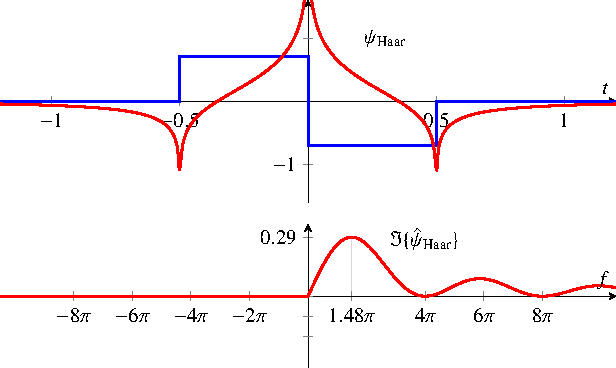
\includegraphics{papers/complex/images/ahaar.pdf}
	\caption{Das analytische Haar-Wavelet im Zeit- und Frequenzbereich.}
	\label{complex:ahaar}
\end{figure}

\begin{figure}
	\centering
	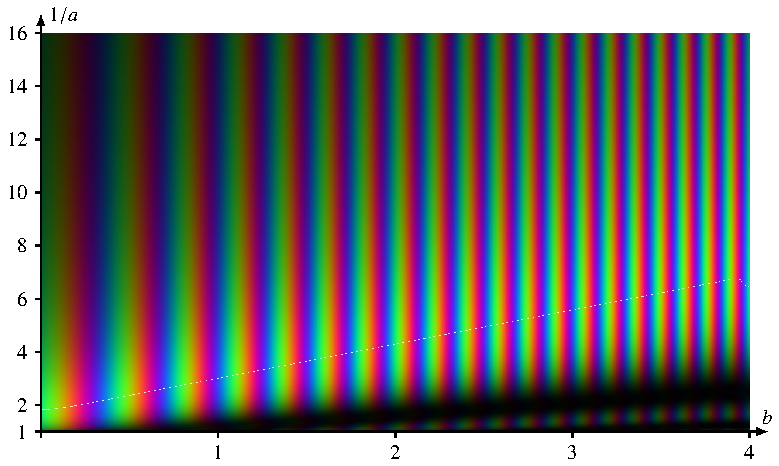
\includegraphics{papers/complex/images/chirp_ahaar.pdf}
	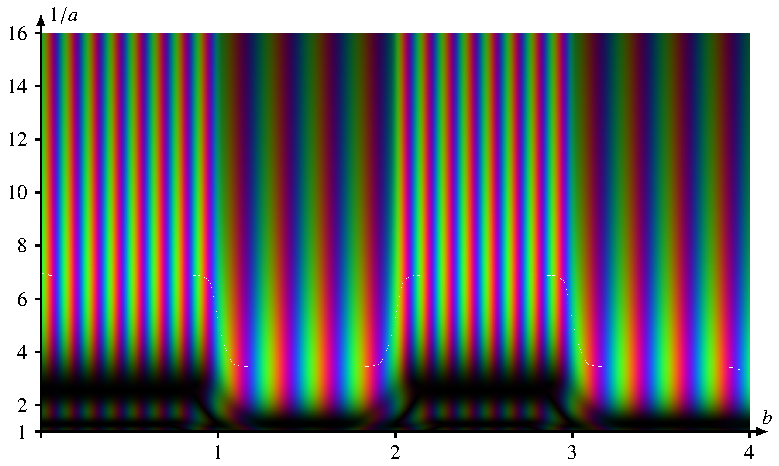
\includegraphics{papers/complex/images/square_ahaar.pdf}
	\caption{Wavelet-Transformationen der beiden Beispielsignale mit dem analytischen Haar-Wavelet. Die Auflösung in der Zeit ist sehr gut, dafür ist die Frequenz nicht ohne Weiteres zu erahnen. Durch die kontinuierliche Amplitude kann man jedoch relativ einfach dem Maximum folgen, um die momentane Frequenz -- skaliert mit $\omega_\psi$ -- zu finden.}
	\label{complex:ahaar-ex}
\end{figure}
